%File: anonymous-submission-latex-2023.tex
\documentclass[letterpaper]{article} % DO NOT CHANGE THIS
\usepackage[submission]{aaai23}  % DO NOT CHANGE THIS
\usepackage{times}  % DO NOT CHANGE THIS
\usepackage{helvet}  % DO NOT CHANGE THIS
\usepackage{courier}  % DO NOT CHANGE THIS
\usepackage[hyphens]{url}  % DO NOT CHANGE THIS
\usepackage{graphicx} % DO NOT CHANGE THIS
\urlstyle{rm} % DO NOT CHANGE THIS
\def\UrlFont{\rm}  % DO NOT CHANGE THIS
\usepackage{natbib}  % DO NOT CHANGE THIS AND DO NOT ADD ANY OPTIONS TO IT
\usepackage{caption} % DO NOT CHANGE THIS AND DO NOT ADD ANY OPTIONS TO IT
\frenchspacing  % DO NOT CHANGE THIS
\setlength{\pdfpagewidth}{8.5in} % DO NOT CHANGE THIS
\setlength{\pdfpageheight}{11in} % DO NOT CHANGE THIS
%
% These are recommended to typeset algorithms but not required. See the subsubsection on algorithms. Remove them if you don't have algorithms in your paper.
\usepackage{algorithm}
\usepackage{algorithmic}

\usepackage{amsmath,amssymb,amsfonts}
\usepackage{graphicx}
\usepackage{textcomp}
\usepackage{xcolor}
\usepackage{booktabs}
\usepackage{stmaryrd}
% \usepackage{algorithmicx}
\usepackage{framed}
\usepackage{enumitem}
% \usepackage[ruled]{algorithm2e}
\usepackage{multirow}
\usepackage{arydshln}
\usepackage{subfigure} % 子图包
% \usepackage{makecell}


%
% These are are recommended to typeset listings but not required. See the subsubsection on listing. Remove this block if you don't have listings in your paper.
\usepackage{newfloat}
\usepackage{listings}
\DeclareCaptionStyle{ruled}{labelfont=normalfont,labelsep=colon,strut=off} % DO NOT CHANGE THIS
\lstset{%
	basicstyle={\footnotesize\ttfamily},% footnotesize acceptable for monospace
	numbers=left,numberstyle=\footnotesize,xleftmargin=2em,% show line numbers, remove this entire line if you don't want the numbers.
	aboveskip=0pt,belowskip=0pt,%
	showstringspaces=false,tabsize=2,breaklines=true}
\floatstyle{ruled}
\newfloat{listing}{tb}{lst}{}
\floatname{listing}{Listing}
%
% Keep the \pdfinfo as shown here. There's no need
% for you to add the /Title and /Author tags.
\pdfinfo{
/TemplateVersion (2023.1)
}

% DISALLOWED PACKAGES
% \usepackage{authblk} -- This package is specifically forbidden
% \usepackage{balance} -- This package is specifically forbidden
% \usepackage{color (if used in text)
% \usepackage{CJK} -- This package is specifically forbidden
% \usepackage{float} -- This package is specifically forbidden
% \usepackage{flushend} -- This package is specifically forbidden
% \usepackage{fontenc} -- This package is specifically forbidden
% \usepackage{fullpage} -- This package is specifically forbidden
% \usepackage{geometry} -- This package is specifically forbidden
% \usepackage{grffile} -- This package is specifically forbidden
% \usepackage{hyperref} -- This package is specifically forbidden
% \usepackage{navigator} -- This package is specifically forbidden
% (or any other package that embeds links such as navigator or hyperref)
% \indentfirst} -- This package is specifically forbidden
% \layout} -- This package is specifically forbidden
% \multicol} -- This package is specifically forbidden
% \nameref} -- This package is specifically forbidden
% \usepackage{savetrees} -- This package is specifically forbidden
% \usepackage{setspace} -- This package is specifically forbidden
% \usepackage{stfloats} -- This package is specifically forbidden
% \usepackage{tabu} -- This package is specifically forbidden
% \usepackage{titlesec} -- This package is specifically forbidden
% \usepackage{tocbibind} -- This package is specifically forbidden
% \usepackage{ulem} -- This package is specifically forbidden
% \usepackage{wrapfig} -- This package is specifically forbidden
% DISALLOWED COMMANDS
% \nocopyright -- Your paper will not be published if you use this command
% \addtolength -- This command may not be used
% \balance -- This command may not be used
% \baselinestretch -- Your paper will not be published if you use this command
% \clearpage -- No page breaks of any kind may be used for the final version of your paper
% \columnsep -- This command may not be used
% \newpage -- No page breaks of any kind may be used for the final version of your paper
% \pagebreak -- No page breaks of any kind may be used for the final version of your paperr
% \pagestyle -- This command may not be used
% \tiny -- This is not an acceptable font size.
% \vspace{- -- No negative value may be used in proximity of a caption, figure, table, section, subsection, subsubsection, or reference
% \vskip{- -- No negative value may be used to alter spacing above or below a caption, figure, table, section, subsection, subsubsection, or reference

\setcounter{secnumdepth}{0} %May be changed to 1 or 2 if section numbers are desired.

% The file aaai23.sty is the style file for AAAI Press
% proceedings, working notes, and technical reports.
%

% Title

% Your title must be in mixed case, not sentence case.
% That means all verbs (including short verbs like be, is, using,and go),
% nouns, adverbs, adjectives should be capitalized, including both words in hyphenated terms, while
% articles, conjunctions, and prepositions are lower case unless they
% directly follow a colon or long dash
\title{PrivNNP: Two-Party Computation Framework for Neural Network Predictions \\ Via a Novel Secret Comparison protocol}
\author{
    %Authors
    % All authors must be in the same font size and format.
    Written by AAAI Press Staff\textsuperscript{\rm 1}\thanks{With help from the AAAI Publications Committee.}\\
    AAAI Style Contributions by Pater Patel Schneider,
    Sunil Issar,\\
    J. Scott Penberthy,
    George Ferguson,
    Hans Guesgen,
    Francisco Cruz\equalcontrib,
    Marc Pujol-Gonzalez\equalcontrib
}
\affiliations{
    %Afiliations
    \textsuperscript{\rm 1}Association for the Advancement of Artificial Intelligence\\
    % If you have multiple authors and multiple affiliations
    % use superscripts in text and roman font to identify them.
    % For example,

    % Sunil Issar, \textsuperscript{\rm 2}
    % J. Scott Penberthy, \textsuperscript{\rm 3}
    % George Ferguson,\textsuperscript{\rm 4}
    % Hans Guesgen, \textsuperscript{\rm 5}.
    % Note that the comma should be placed BEFORE the superscript for optimum readability

    1900 Embarcadero Road, Suite 101\\
    Palo Alto, California 94303-3310 USA\\
    % email address must be in roman text type, not monospace or sans serif
    publications23@aaai.org
%
% See more examples next
}

%Example, Single Author, ->> remove \iffalse,\fi and place them surrounding AAAI title to use it
\iffalse
\title{My Publication Title --- Single Author}
\author {
    Author Name
}
\affiliations{
    Affiliation\\
    Affiliation Line 2\\
    name@example.com
}
\fi

\iffalse
%Example, Multiple Authors, ->> remove \iffalse,\fi and place them surrounding AAAI title to use it
\title{My Publication Title --- Multiple Authors}
\author {
    % Authors
    First Author Name,\textsuperscript{\rm 1}
    Second Author Name, \textsuperscript{\rm 2}
    Third Author Name \textsuperscript{\rm 1}
}
\affiliations {
    % Affiliations
    \textsuperscript{\rm 1} Affiliation 1\\
    \textsuperscript{\rm 2} Affiliation 2\\
    firstAuthor@affiliation1.com, secondAuthor@affilation2.com, thirdAuthor@affiliation1.com
}
\fi


% REMOVE THIS: bibentry
% This is only needed to show inline citations in the guidelines document. You should not need it and can safely delete it.
\usepackage{bibentry}
% END REMOVE bibentry

\begin{document}

\maketitle

\begin{abstract}

    Deep learning has achieved overwhelming successes in many fields, including image classification, speech recognition, machine translation etc.
    A pre-trained deep neural network model can predict the outcomes
    for a given data point. Such a deep neural network model can be served by
    specialized AI companies to users as a cloud prediction services.
    However, such a service model faces a privacy dilemma: neither AI companies nor
    users want to expose their private information.
    To achieve both model privacy and input data privacy,
    secure multi-party computation can utilized to evaluate prediction outcomes. However,
    this strategy is further complicated due to the complex deep learning prediction process.
    Currently, all existing solutions are very inefficient for employing complex asymmetric cryptographic operations.

    We propose PrivNNP, a two-party computation (2PC) framework for efficient neural network predictions.
    PrivNNP is highly efficient because it does not use any asymmetric cryptography to simultaneously preserve model privacy and input data privacy.
    The core of PrivNNP is a novel and efficient two-party comparison protocol,
    which consists of three rounds of interactions without any oblivious transfer.
    From this building block, we construct the complete scheme for evaluating layers of the neural network, including the convolution layer, the pooling layer and the activation function.
	We formally prove that PrivNNP is {\bf secure} and also fully implement it with Python.
    Comprehensive experiments show that PrivNNP on resnet50
    costs only 23.86 seconds in computation and 100.13 seconds in communication.


\end{abstract}


\section{Introduction}



    \noindent Deep learning, a popular research direction in the field of machine learning,
    has brought major breakthroughs to computer vision, speech recognition, natural language process, machine translation, etc. Recently,
    deep learning also made significant progress in bioinformatics, drug discovery and material sciences.
    A deep neural network model is obtained by training on
	a given training data set, which requires a large amount of training data and sufficient compute power.
	After the training step, the resultant deep neural network model is used to predict
	outcomes for a given data point. It is important to protect both the training phase and the predicting phase,
    while this work mainly focuses on the prediction phase.

    Deep learning models can be serviced on cloud by the model owner as a cloud-based service,
    i.e. Machine Learning as a Service (MLaaS),
    which consists of a series of machine learning tools offered by cloud service providers \cite{ChironCloud}.
    Computationally intensive tasks that cannot be accomplished by data owners can be outsourced to
    the MLaaS cloud hosting the pre-trained deep learning model.
    For example, the computed tomography (CT) images of a patient taken by hospitals
    can be sent to the MLaaS cloud for medical diagnosis.
    However, MLaaS faces two types of privacy leakage problems, namely the model privacy leakage and the
    input data privacy leakage. That is, the model owner has to send all the model parameters to the hosting cloud,
    while the patient has to surrender his/her CT images during this process.

    To address this issue, secure multi-party computation (MPC) can be employed to preserve both the model privacy
    and the input data privacy in deep learning prediction.
    Generally, MPC enables multiple participants
    to compute outputs from their private inputs without leaking privacy.
    A particular case of MPC, the two-party computation (2PC) setting
    which only involves two parties, is used throughout the paper.

    The biggest challenge of the 2PC framework
    is the large cost during implementing the system.
    Existing works usually utilize asymmetric cryptography like oblivious transfer and garbled circuits
    to preserve privacy for deep learning,
    leading to prohibitive computation cost.


    \subsection{Our contributions}%%%%%%%%%%%%%%%%%%%%%%%%%%%%%%%%%%%%%%%%%%%%%%%%%%%%%%%%%%%%%%%%%%%%%%%%%%%%%%%%%%%%%%%%%%%%%%%%%%%%
    Here we summarize our contributions.

    \begin{itemize}
        \item \textbf{PrivNNP}.
        We present PrivNNP, an efficient two-party computation framework
        for evaluating neural network predictions.

        The building block of our work is a brand new 2PC-$\mathtt{comparison}$ protocol,
        which does not utilize the asymmetric cryptography or the bit-level operations
        and only consists of three rounds of interactions to calculate the sign of the secret input value.
        The computation is $l\times$ faster than the Sharemind \cite{Sharemind}
        when the the secret input is a $l-$bit value.
        % Equiped with the novel 2PC-$\mathtt{comparison}$ protocol, we design schemes for more complicated functions
        % like maximum function and piecewise functions.
        \item \textbf{Security analysis}.
        We theoretically prove that our system satisfies the
        security definition of the two-party computation.

        \item \textbf{Experiment}.
        To demonstrate the performance of our work,
        we implement PrivNNP and conduct experiment on the classical
        neural network model Resnet50 and
        it costs 23s for computation and 100s for communication.

   \end{itemize}

\section{Related Work}
    Many ideas have been proposed to achieve privacy-preserving neural network predictions.
    The most common idea is to utilize fully homomorphic encryption  \cite{SEAL} \cite{Homomorphic1}
    which supports multiplication and addition on ciphertexts.
    The data owner sends the encrypted image to the model provider for applying a pre-trained model for classification \cite{FullyHomomorphic}.
    Furthermore, some proposals that only use additive homomorphic encryption are presented \cite{Homomorphic2}.
    However, the overhead of homomorphic encryption is so large that
    the cost of it seems still unacceptable
    though the associated technology evolves over many years\cite{ObliviousNeuralNetwork}, .

    To reduce the overhead of homomorphic encryption operations,
    some more efficient schemes for MPC operations are presented.
    On a very high level, the MPC multiplication is easy to be implemented by the Beaver triple \cite{EfficientMultipartyProtocols}
    but the MPC comparison is very hard to realize.
    To avoid the expensive cost of comparison,
    a modified deep learning model \cite{CryptoNets} using square activation function and the mean pooling so that
    no comparison operation is needed in MPC neural network.
    Obviously, this architecture has a narrow application scope.

    In order to realize practical comparison protocol, ABY framework \cite{ABY} is proposed
    and then be extended to ABY3 \cite{ABY3} which can be performed among 3 parties.
    Both ABY and ABY3 involve the asymmetric cryptography
    including the oblivious transfer protocol and the garbled circuit.
    Up to this day, most of the systems \cite{2022GarbledCircuit} still keep tring to optimizing
    the garbled circuit process to lower the communication and computation complexity.
    Sharemind \cite{Sharemind} provides a new idea that converts a comparison operation to
    multi-round bit-level multiplication.
    Though it lowers the computational difficulty, it costs too much rounds for
    communication.

\section{Preliminaries}
    \subsection{Notations}

    \begin{table}
        \resizebox{0.45\textwidth}{!}{
        \begin{tabular}{l||l}
            \hline
            \hline
            $\mathcal{DO}$ & Data owner\\
            $\mathcal{MP}$ & Model provider\\
            $\mathcal{TTP}$ & The trusted setup\\
            $\mathcal{P}_{0},\mathcal{P}_{1}$ & Two parties who run PrivNNP\\
            $\mathcal{P}_{i}$ & The $i$-th party, $i\in \{0,1\}$\\
            $\langle x\rangle$ & Additively shared value $x$\\
            $\langle x\rangle^{i}$ & Additive share of value $x$ held by $\mathcal{P}_{i},i\in \{0,1\}$ \\
            $\llbracket x \rrbracket$ & Multiplicatively shared value $x$\\
            $\llbracket x \rrbracket^{i}$ & Multiplicative share of value $x$ held by $\mathcal{P}_{i},i\in \{0,1\}$\\
            $\otimes $ & 2PC-multiplication operation performed on shares\\
            $(\langle a\rangle,\langle b\rangle,\langle c\rangle)$ & Multiplication triple\\
            $(\langle \mathbf{A}\rangle,\langle \mathbf{B}\rangle,\langle \mathbf{C}\rangle)$ & Matrix multiplication triple\\
            $(\langle u\rangle,\llbracket u \rrbracket)$ & Comparison bigram \\
            \hline
            \hline
        \end{tabular}}
        \caption{Notations}
        \label{Notations}
    \end{table}
    Notations used in this paper is listed in Table \ref{Notations}.
    In addition, a matrix is denoted by bold capital letters (e.g. $\mathbf{A}$) and
    a vector is denoted as $\overrightarrow{\mathbf{v}}=(v_{0},v_{1},...,v_{n-1})$ .

    Function $\mathsf{sign}(x)$ is defined to represent the sign of value $x$.
    Note that, $\mathsf{sign}(x\cdot y)=\mathsf{sign}(x)\cdot \mathsf{sign}(y)$.
    $$\mathsf{sign}(x)=\begin{cases}
        1 & \text{ if } x>0 \\
        0 & \text{ if } x=0\\
        -1 & \text{ if } x<0
    \end{cases}$$

    \subsection{Multi-Party Computation and Two-Party Computation}
    MPC enables multiple participants to jointly compute a function over their private inputs without leaking
	their individual input. It has broad applications where privacy is important, e.g. voting, auction,
	data mining etc. Two-party computation (2PC) is a special case of MPC.
    In this work, we consider semi-honest 2PC participants
    who will not deviate from the protocol but may try to gain private information of another party
		during the protocol execution.

    \subsection{2PC secret sharing}
    % Secret sharing is a method that a secret is split in some ways and each share is held by each participant    and
    2PC secret sharing means a secret value is shared between two parties.
    Our framework involves two types of 2PC secret sharing methods:
    additive sharing and multiplicative sharing.
    \begin{itemize}
        \item
        The additively shared secret value $x$ is denoted as $\langle x\rangle $.
        When two parties additively share value $x$,
        each party $\mathcal{P}_{i}$ holds the secret share as $\langle x\rangle ^{i}$, s.t.
        $x=\langle x\rangle ^{0}+\langle x\rangle ^{1}$.

        Similarly, $\langle \mathbf{A}\rangle $ is used to indicate an additively shared secret matrix
        and $\mathbf{A} =\langle \mathbf{A}\rangle ^{0}+\langle \mathbf{A}\rangle ^{1}$.

        \item The multiplicatively shared secret value $x$ is denoted as $\llbracket x \rrbracket$.
        When parties multiplicatively share the secret value $x$,
        each party $\mathcal{P}_{i}$ holds the secret share as $\llbracket x \rrbracket ^{i}$, s.t.
        $x=\llbracket x \rrbracket ^{0}\times \llbracket x \rrbracket ^{1}$.

    \end{itemize}


    All protocols we present operate on shares, which means
    the input and the output of these protocols are hidden for all parties.
    For instance, we use $\otimes$ to represent the multiplication between two additively shared value.
    When performing multiplication operations on shares,
    we write $\langle z\rangle=\langle x\rangle\otimes  \langle y\rangle $,
    which means that the two parties compute the product of two additively shared value
    $\langle x\rangle, \langle y\rangle$ and obtaining the
    the additive share of the product.
    $\mathcal{P}_{i}$ can only get the value of $\langle x\rangle ^{i}$, $\langle y\rangle ^{i}$ and $\langle z\rangle ^{i}$ ($i \in \{0,1\}$).
    This enable two parties to run multiple rounds of different protocols while keeping secret state input.

    \subsection{Auxiliary tuples}
    Some auxiliary tuples of specific structures are used to
    assit in running $\mathtt{multiplication}$ and $\mathtt{comparison}$ protocols.
    These tuples will be generated by the trusted setup and be distributed to each party.
    \begin{itemize}
        \item Multiplication triple: $(\langle a\rangle,\langle b\rangle,\langle c\rangle)$, where $c=a\cdot b$.
        \item Matrix multiplication triple: $(\langle \mathbf{A}\rangle,\langle \mathbf{B}\rangle,\langle \mathbf{C}\rangle)$, where $\mathbf{C}=\mathbf{A}\cdot \mathbf{B}$.
        \item Comparison bigram: $(\langle u\rangle,\llbracket u \rrbracket)$,
        this bigram consists of the additive share and the multiplicative share of the same value $u$ ($u\neq 0 $).
    \end{itemize}


    \subsection{Layers of neural networks}
    A neural network consists of a pipeline of layers which can be mainly divided into three categories:
    convolution layer, pooling layer and activation function layer.
    % Here we briefly introduce the layers of neural network.
    \begin{itemize}
        \item \textbf{Convolution layer:}
        Convolution is an operation between the imput image and the filter.
        It computes the dot product of the filter and the corresponding submatrix in the input image.
        This step is repeated by sliding the filter to get the output matrix.
        To improve the efficiency, convolution is usually converted to matrix multiplication and addition.

        \item \textbf{Pooling layer:}
        Pooling layer is calculated by $n\times n$ size matrix sliding window.
        There are two types of pooling layer: average pooling and maximum pooling,
        which outputs the average or the maximum of $n\times n$ size matrices to construct the input matrix of the next layer.

        \item \textbf{Activation function layer:}
        Activation function is a function acting on the neuron of the artificial neural network,
        mapping the input of the neuron to the output.
        Common used activation functions are listed as follow:
        \begin{align*}
        \text{Maxout:} \mathsf{f}(x) &= \mathsf{max}( \overrightarrow{\mathbf{x}})\\
        \text{Sigmoid:} \sigma(x) &=\frac{1}{1+e^{-x}}\\
        \mathsf{ReLU}(x)&=\begin{cases}
            x & \text{ if } x > 0 \\
            0 & \text{ if } x \leqslant 0 \\
            \end{cases}
        \end{align*}
        In the paper, we mainly introduce method to compute $\mathsf{ReLU}$ function.
        Other functions can be computed by similar approach.
    \end{itemize}
    The PrivNNP will include 2PC-algorithms for evaluating each layer.

\section{Two-party Secure Computation for Basic Operations}

    In this section we introduce 2PC protocols for basic operations,
    including addition, comparison, maximum and piecewise function.
    Our protocols all operate on shares, which means
    the input and the output is in the form of additive shares.
    This enables two parties to run multiple rounds of different
    protocols while keeping the input secret
    and facilitate further processing to implement a complex system.

    % Formalized protocols are presented in the appendix.

    \subsection{Addition}

    \emph{Computing} $ \langle z\rangle  = \langle x\rangle  + \langle y\rangle $. This operation can be done without interaction by
    $\mathcal{P}_{i}$ setting $\langle z\rangle^{i}  = \langle x\rangle^{i}  + \langle y\rangle^{i} $.

    \begin{figure}[ht]
        % \centering{\bf Two-party secure computation protocol for operations}
        \resizebox{0.48\textwidth}{!}{
        \begin{tabular}{lcl}
            \hline
            \multicolumn{3}{c}{\underline{$\mathtt{Addition }$}:}\\
            \multicolumn{3}{l}{\textbf{Target}: compute $\langle z\rangle  = \langle x\rangle  + \langle y\rangle $}\\
            \textbf{Input}:\\
            $\mathcal{P}_{0}$ &  &  $\mathcal{P}_{1}$ \\
            $\{(\langle x\rangle ^{0} , \langle y\rangle ^{0})\}$,
            &~~~~~~~~~~~~~~~~~~~~~~~~~~~~~~~~~~~~~~~~~~~~~~~~
            &
            $\{(\langle x\rangle ^{1} , \langle y\rangle ^{1})\}$,

            \\

            \textbf{Procedure}:\\
            $\mathcal{P}_{0}$ &  &  $\mathcal{P}_{1}$ \\
            $\langle z\rangle ^{0}\leftarrow\langle x\rangle ^{0}+\langle y\rangle ^{0}$
            &
            &
            $\langle z\rangle ^{1}\leftarrow\langle x\rangle ^{1}+\langle y\rangle ^{1}$
            \\
            \hline

        \end{tabular}}
        \caption{2PC-addition}
        \label{2PC-addition}
    \end{figure}
    The 2PC-addition protocol is shown in Figure \ref{2PC-addition}.

    \subsection{Multiplication}
    \emph{Computing} $ \langle z\rangle  = \langle x\rangle  \otimes \langle y\rangle $.
    $\mathtt{Multiplication}$ protocol is used to compute the product of two shared values
    and is performed using a auxiliary multiplication triple
    $(\langle a\rangle,\langle b\rangle,\langle c\rangle)$,
    which can be distributed from the trusted third party.
    \begin{figure}[ht]
        % \centering{\bf Two-party secure computation protocol for operations}
        \resizebox{0.48\textwidth}{!}{
        \begin{tabular}{lcl}
            \hline
            \multicolumn{3}{c}{\underline{$\mathtt{Multiplication}$}:}\\
            \multicolumn{3}{l}{\textbf{Target}: compute $\langle z\rangle  = \langle x\rangle  \otimes \langle y\rangle $}\\
            % \textbf{Target}: compute $\langle z\rangle  = \langle x\rangle  \cdot \langle y\rangle $\\
            \textbf{Input}:\\
            % & \hfil\underline{$\mathtt{Multiplication}$}:\hfil\\
            $\mathcal{P}_{0}$ &  &  $\mathcal{P}_{1}$ \\
            $\{(\langle x\rangle ^{0} , \langle y\rangle ^{0})$,
            &
            &
            $\{(\langle x\rangle ^{1} , \langle y\rangle ^{1})$,

            \\

            mul-triple:$
            (\langle a\rangle ^{0},\langle b\rangle ^{0},\langle c\rangle ^{0})\}$
            &
            &
            mul-triple:$ (\langle a\rangle ^{1},\langle b\rangle ^{1},\langle c\rangle ^{1})\}$
            \\
            \textbf{Procedure}:\\
            $\mathcal{P}_{0}$ &  &  $\mathcal{P}_{1}$ \\
            $\langle e\rangle ^{0}\leftarrow\langle x\rangle ^{0}-\langle a\rangle ^{0}$
            &
            &
            $\langle e\rangle ^{1}\leftarrow\langle x\rangle ^{1}-\langle a\rangle ^{1}$
            \\
            $\langle f\rangle ^{0}\leftarrow\langle y\rangle ^{0}-\langle b\rangle ^{0}$
            &
            &
            $\langle f\rangle ^{1}\leftarrow\langle y\rangle ^{1}-\langle b\rangle ^{1}$
            \\
            & $\underrightarrow{~~~~~~(\langle e\rangle ^{0},\langle f\rangle ^{0})~~~~~~}$ &\\
            & $\underleftarrow{~~~~~~(\langle e\rangle ^{1},\langle f\rangle ^{1})~~~~~~}$ &\\
            $e\leftarrow\langle e\rangle ^{0}+\langle e\rangle ^{1}$& &$e\leftarrow\langle e\rangle ^{0}+\langle e\rangle ^{1}$\\
            $f\leftarrow\langle f\rangle ^{0}+\langle f\rangle ^{1}$& &$f\leftarrow\langle f\rangle ^{0}+\langle f\rangle ^{1}$\\
            $\langle z\rangle^{0}\leftarrow f\cdot \langle a\rangle^{0}$
            & &
            $\langle z\rangle^{1}\leftarrow e \cdot f + f\cdot \langle a\rangle^{1}$\\
            $+e \cdot \langle b\rangle^{0} + \langle c\rangle^{0}$& &$+e \cdot \langle b\rangle^{1} + \langle c\rangle^{1}$\\
            \hline

        \end{tabular}}
        \caption{2PC-multiplication}
        \label{2PC-multiplication}


    \end{figure}
    The 2PC-multiplication protocol is shown in Figure \ref{2PC-multiplication}.

    Moreover, if the private input data is not in the share state,
    such as $\mathcal{P}_{0}$ holding the secret value $x$
    and $\mathcal{P}_{1}$ holding the secret value $y$.
    In this situation, the value $x$ and $y$ can be
    seen as a special share state, where
    $\langle x\rangle ^{0}=x,\langle x\rangle ^{1}=0$ and
    $\langle y\rangle ^{0}=0,\langle y\rangle ^{1}=y$.

    They can compute $\langle z\rangle=x\otimes y$ secretly
    by running $\mathtt{multiplication}$ protocol with the special input of
    $\mathcal{P}_{0}:(x,0),\mathcal{P}_{1}:(0,y)$.



    \begin{figure}[ht]
        % \centering{\bf Two-party secure computation protocol for operations}
        \resizebox{0.48\textwidth}{!}{
        \begin{tabular}{lcl}
            \hline
            \multicolumn{3}{c}{\underline{$\mathtt{Matrix \enspace multiplication}$}:}\\
            \multicolumn{3}{l}{\textbf{Target}: compute $\langle \mathbf{Z}\rangle  = \langle \mathbf{X}\rangle  \otimes \langle \mathbf{Y}\rangle $}\\
            \textbf{Input}:\\
            % & \hfil\underline{$\mathtt{Multiplication}$}:\hfil\\
            $\mathcal{P}_{0}$ &  &  $\mathcal{P}_{1}$ \\
            $\{(\langle \mathbf{X}\rangle ^{0} , \langle \mathbf{Y}\rangle ^{0})$,
            &
            &
            $\{(\langle \mathbf{X}\rangle ^{1} , \langle \mathbf{Y}\rangle ^{1})$,

            \\

            mul-triple:$
            (\langle \mathbf{A}\rangle ^{0},\langle \mathbf{B}\rangle ^{0},\langle \mathbf{C}\rangle ^{0})\}$
            &
            &
            mul-triple:$ (\langle \mathbf{A}\rangle ^{1},\langle \mathbf{B}\rangle ^{1},\langle \mathbf{C}\rangle ^{1})\}$
            \\
            \textbf{Procedure}:\\
            $\mathcal{P}_{0}$ &  &  $\mathcal{P}_{1}$ \\
            $\langle \mathbf{E}\rangle ^{0}\leftarrow\langle \mathbf{X}\rangle ^{0}-\langle \mathbf{A}\rangle ^{0}$
            &
            &
            $\langle \mathbf{E}\rangle ^{1}\leftarrow\langle \mathbf{X}\rangle ^{1}-\langle \mathbf{A}\rangle ^{1}$
            \\
            $\langle \mathbf{F}\rangle ^{0}\leftarrow\langle \mathbf{Y}\rangle ^{0}-\langle \mathbf{B}\rangle ^{0}$
            &
            &
            $\langle \mathbf{F}\rangle ^{1}\leftarrow\langle \mathbf{Y}\rangle ^{1}-\langle \mathbf{B}\rangle ^{1}$
            \\
            & $\underrightarrow{~~~~~~(\langle \mathbf{E}\rangle ^{0},\langle \mathbf{F}\rangle ^{0})~~~~~~}$ &\\
            & $\underleftarrow{~~~~~~(\langle \mathbf{E}\rangle ^{1},\langle \mathbf{F}\rangle ^{1})~~~~~~}$ &\\
            $e\leftarrow\langle \mathbf{E}\rangle ^{0}+\langle \mathbf{E}\rangle ^{1}$& &$\mathbf{E}\leftarrow\langle \mathbf{E}\rangle ^{0}+\langle \mathbf{E}\rangle ^{1}$\\
            $f\leftarrow\langle \mathbf{F}\rangle ^{0}+\langle \mathbf{F}\rangle ^{1}$& &$\mathbf{F}\leftarrow\langle \mathbf{F}\rangle ^{0}+\langle \mathbf{F}\rangle ^{1}$\\
            $\langle \mathbf{Z}\rangle^{0}\leftarrow \mathbf{F}\cdot \langle \mathbf{A}\rangle^{0}$
            & &
            $\langle \mathbf{Z}\rangle^{1}\leftarrow \mathbf{E} \cdot \mathbf{F} + \mathbf{F}\cdot \langle \mathbf{A}\rangle^{1}$\\
            $+\mathbf{E} \cdot \langle \mathbf{B}\rangle^{0} + \langle \mathbf{C}\rangle^{0}$& &$+\mathbf{E} \cdot \langle \mathbf{B}\rangle^{1} + \langle \mathbf{C}\rangle^{1}$\\
            \hline

        \end{tabular}}
        \caption{2PC-matrix multiplication}
        \label{2PC-matrix_multiplication}


    \end{figure}
    \emph{Computing} $ \langle \mathbf{Z}\rangle  = \langle \mathbf{X}\rangle  \otimes \langle \mathbf{Y}\rangle$.
    Similarly, there is a protocol for the 2PC-matrix multiplication, as shown in Figure \ref{2PC-matrix_multiplication}.

    \subsection{Comparison}
    The 2PC-$\mathtt{comparison}$ protocol is the most important building block of our work.
    Two questions will be discussed in this subsection:
    how to compute $\mathsf{sign}(x)$ and $\mathsf{max}(x,y)$ via 2PC protocols.


    \emph{Computing} $\langle s\rangle  = \langle \mathsf{sign}(\langle x\rangle)\rangle $.
    The $\mathtt{comparison}$ protocol for computing the sign of the shared value utilizes the comparison bigram $(\langle u\rangle,\llbracket u \rrbracket )$.

    In our scheme, the two parties first compute $ \langle z\rangle = \langle x\rangle\otimes \langle u\rangle$
    via $\mathtt{multiplication}$ protocol
    to blind the value of $x$.
    Then, $\mathcal{P}_{1}$ sends  $ \langle z\rangle^{1}$ to $\mathcal{P}_{0}$ and
    $\mathcal{P}_{0}$ reconstructs the true value of $z$.
    Note that
    $$x=\frac{x\cdot u}{u}
    %    = \frac{x\cdot u}{q}
        =\frac{z\cdot 1}{\llbracket u \rrbracket^{0}\cdot \llbracket u \rrbracket^{1}}
        =\frac{z}{\llbracket u \rrbracket^{0}}\cdot\frac{1}{\llbracket u \rrbracket^{1}}$$

    Recall that $\mathsf{sign}(x\cdot y)=\mathsf{sign}(x)\cdot \mathsf{sign}(y)$, so
    $$\mathsf{sign}(x)=\frac{\mathsf{sign}(x \cdot u)}{\mathsf{sign}(u)}
    % =\frac{\mathsf{sign}(z)}{\mathsf{sign}(u)}
    =\mathsf{sign}(\frac{z}{\llbracket u \rrbracket^{0}})
    \cdot \mathsf{sign}(\frac{1}{\llbracket u \rrbracket^{1}})$$

    Because the $(\llbracket u \rrbracket^{0},z)$ and $\llbracket u \rrbracket^{1}$
    is held by $\mathcal{P}_{0}$ and $\mathcal{P}_{1}$ respectively.
    Therefore, the multiplicative share of $\mathsf{sign}(x)$ can be obtained by
    $\mathcal{P}_{0}$ setting $\llbracket s \rrbracket^{0}
    =\mathsf{sign}(\frac{z}{\llbracket u \rrbracket^{0}})$
    and $\mathcal{P}_{1}$ setting $\llbracket s \rrbracket^{1}
    =\mathsf{sign}(\frac{1}{\llbracket u \rrbracket^{1}})$ locally
    so that $\mathsf{sign}(x)=\llbracket s \rrbracket^{0}\cdot \llbracket s \rrbracket^{1}$.

    In order to compute more complicated functions,
    the multiplicative share $\llbracket s \rrbracket$ should be converted into the additive share $\langle s\rangle$
    by calculating $\langle s\rangle = \llbracket s \rrbracket ^{0}\otimes \llbracket s \rrbracket ^{1}$.
    More precisely, two parties run $\mathtt{multiplication}$ protocol with the input of
    $\mathcal{P}_{0}:(\llbracket s \rrbracket ^{0},0),\mathcal{P}_{1}:(0,\llbracket s \rrbracket ^{1})$, and
    \begin{align*}
        \langle s\rangle^{0} +\langle s\rangle^{1}&=(\llbracket s \rrbracket ^{0}+0)\otimes (0+\llbracket s \rrbracket ^{1})\\
        &=\llbracket s \rrbracket ^{0}\cdot \llbracket s \rrbracket ^{1}=\mathsf{sign}(x)
    \end{align*}
    \begin{figure}[ht]
        \resizebox{0.48\textwidth}{!}{
        \begin{tabular}{lcl}
            \hline
            \multicolumn{3}{c}{\underline{$\mathtt{Comparison}$}:}\\
            \textbf{Computation for $\mathsf{sign}(x)$}:&&\\
            \textbf{Target}: compute $\langle s\rangle  = \langle \mathsf{sign}(\langle x \rangle )\rangle $\\
            \textbf{Input}:\\
            $\mathcal{P}_{0}$ &  &  $\mathcal{P}_{1}$ \\
            $\{\langle x\rangle ^{0}$,
            &
            &
            $\{\langle x\rangle ^{1}$,

            \\

            comp-bigram:$
            (\langle u\rangle ^{0},\llbracket u \rrbracket ^{0})\}$
            &
            &
            comp-bigram:$ (\langle u\rangle ^{1},\llbracket u \rrbracket ^{1})\}$\\
            \textbf{Procedure}:\\
            $\mathcal{P}_{0}$ &  &  $\mathcal{P}_{1}$ \\
            \hdashline
            \multicolumn{3}{c}{run $\mathtt{multiplication}$ protocol to}\\
            \multicolumn{3}{c}{$\text{compute }
            \langle z\rangle = \langle u\rangle \otimes \langle x\rangle $ }\\
            gets $\langle z\rangle ^{0}$& &gets $\langle z\rangle ^{1}$\\

            \hdashline
            & $\underleftarrow{~~~~~\langle z\rangle ^{1}~~~~~}$~~~~~ &\\
            $z\leftarrow\langle z\rangle ^{0}+\langle z\rangle ^{1}$& &\\
            $\llbracket s \rrbracket^{0}
            \leftarrow \mathsf{sign}(\frac{1}{\llbracket u \rrbracket^{0}})$&
            &$\llbracket s \rrbracket^{1}
            \leftarrow \mathsf{sign}(\frac{z}{\llbracket u \rrbracket^{1}})$\\

            \hdashline
            \multicolumn{3}{c}{run $\mathtt{multiplication}$ protocol to}\\
            \multicolumn{3}{c}{compute $
            \langle s\rangle = \llbracket s \rrbracket ^{0} \otimes \llbracket s \rrbracket ^{1}$}\\

            gets $\langle s\rangle ^{0}$& &gets $\langle s\rangle ^{1}$\\
            \hdashline
            \hline
        \end{tabular}}
        \caption{2PC-comparison}
        \label{2PC-comparison}
    \end{figure}
    2PC-comparison protocol is shown in Figure \ref{2PC-comparison}.

    \textbf{Security analysis}:
       Throughout our $\mathtt{comparison}$ protocol,
       it uses two $\mathtt{multiplication}$ protocol and disclose one blinded value.
       Since $\mathtt{multiplication}$ protocol is proposed by previous work
       and the security of it has been proved, our $\mathtt{comparison}$ protocol is secure
       and satisfy the definition of
       For space limitation, more details can be seen in supplementary material.



       \emph{Computing} $ \langle maximum\rangle  = \langle \mathsf{max}(\langle x\rangle,\langle y\rangle)\rangle $.
       This part aims at providing a method to compute the maximum of two shared values $\langle x \rangle$ and $\langle y \rangle$.
       It is easy to see that
       $$\mathsf{max}(x,y) = \left\{\begin{matrix}
           x & x>y\\
           \frac{x+ y}{2} & x=y\\
           y & x<y
           \end{matrix}\right.$$
       Let $s = \mathsf{sign}(x-y)$, which means
       $$s = \left\{\begin{matrix}
           1 & x>y\\
           0 & x=y\\
           -1 & x<y
           \end{matrix}\right.$$
       We can combine two expressions into one:
       $$\mathsf{max}(x,y) = \frac{(s+1)\cdot x+ (-s+1)\cdot y}{2}$$

       \begin{figure}[ht]
        \resizebox{0.48\textwidth}{!}{
        \begin{tabular}{lcl}
            \hline
            \multicolumn{3}{l}{\textbf{Computation for $\mathsf{max}(x)$}:}\\
            \multicolumn{3}{l}{\textbf{Target}: compute $\langle maximum\rangle  = \langle \mathsf{max}(\langle x\rangle,\langle y\rangle)\rangle$}\\
            \textbf{Input}:\\
            $\mathcal{P}_{0}$ &  &  $\mathcal{P}_{1}$ \\
            $\{\langle x\rangle ^{0} , \langle y\rangle ^{0}\}$
            &
            &
            $\{\langle x\rangle ^{1} , \langle y\rangle ^{1}\}$
            \\
            \textbf{Procedure}:\\
            $\mathcal{P}_{0}$ &  &  $\mathcal{P}_{1}$ \\
            $\langle \Delta\rangle ^{0} \leftarrow \langle x\rangle^{0}-\langle y\rangle^{0}$
            & ~~~~~~~~~~~~~~~~~~~~~~~~~~~~~~~~~~~~&
            $\langle \Delta\rangle ^{1} \leftarrow \langle x\rangle^{1}-\langle y\rangle^{1}$\\
            \hdashline
            \multicolumn{3}{c}{run $\mathtt{comparison}$ protocol to}\\
            \multicolumn{3}{c}{compute
            $\langle s\rangle=\mathsf{sign}(\langle \Delta\rangle)$}\\
            gets $\langle s\rangle ^{0}$& &gets $\langle s\rangle ^{1}$\\
            \hdashline
            \hdashline
            \multicolumn{3}{c}{run $\mathtt{multiplication}$ protocol to}\\
            \multicolumn{3}{c}{compute
            $\langle maximum\rangle=\frac{(\langle s\rangle+1)\otimes \langle x\rangle+ (-\langle s\rangle+1)\otimes \langle y\rangle}{2}$}\\
            gets $\langle maximum\rangle ^{0}$& &gets $\langle maximum\rangle ^{1}$\\
            \hdashline
            \hline
        \end{tabular}}

        \caption{2PC-maximum}
        \label{2PC-max}
    \end{figure}
    Following this idea, the whole process of 2PC-comparison protocol is shown in Figure \ref{2PC-max}.

    Furthermore, we explore variations of $\mathsf{max}(x,y)$.
    Firstly, maximum of a vector $\mathsf{max}(\overrightarrow{\mathbf{x}})=\mathsf{max}(x_{0},x_{1},...x_{n})$
    can be computed by recursively running $\mathtt{comparison}$ protocol.
    % Observing that
    % \begin{align*}
    %     \mathsf{max}(x_{0},x_{1},...x_{n}) &= \mathsf{max}(x_{0},\mathsf{max}(x_{1},x_{2},...x_{n})) \\
    %     &= \mathsf{max}(x_{0},\mathsf{max}(x_{1},...\mathsf{max}(x_{n-1},x_{n})))
    % \end{align*}
    % So the maximum of vector $\overrightarrow{\mathbf{x}}$

    Secondly, because of $\mathsf{min}(x,y)=-\mathsf{max}(-x,-y)$,  $min(x,y)$ can also be computed.
    Combined with the above methods,
    any composite function constructed of $\mathsf{max}()$ and $min()$ can be computed following rules metioned above.


    \subsection{Continuous piecewise function}
    \emph{Computing} $\langle value\rangle  = \langle \mathsf{F}(\langle x\rangle)\rangle $.
    $\mathsf{F}()$ is a public continuous piecewise function constructed by a series of sub-functions $\mathsf{f}_{j}(x)$
    with dividing points $-\infty =d_{0}<d_{1}<...<d_{j}<...<d_{n}=+\infty$.
    When $d_{j-1}< x\leq d_{j}$, $\mathsf{F}(x) =\mathsf{f}_{j}(x)$.
    Since $\mathsf{F}()$ is a continuous function, $\mathsf{F}(d_{j}) =\mathsf{f}_{j}(d_{j})=\mathsf{f}_{j+1}(d_{j})=\frac{\mathsf{f}_{j}(d_{j})+\mathsf{f}_{j+1}(d_{j})}{2}$.


    To solve this problem, we need to compute a vector of
    $\overrightarrow{v}=(v_{0},v_{1},...,v_{n-1})$ to represent which span is $x$ in.
    Let $v_{j} = \frac{1-\mathsf{sign}(d_{j-1}-x)\cdot \mathsf{sign}(d_{j}-x)}{2}$.
    In view of $-\infty =d_{0}$ and $d_{n}=+\infty$,
    we set $\mathsf{sign}(d_{0}-x)=-1$ and $\mathsf{sign}(d_{n}-x)=1$.
    It is easy to see that
    $$v_{j}=\begin{cases}
        0 & \text{ if } x\notin (d_{j-1},d_{j}) \\
        \frac{1}{2} & \text{ if } x = d_{j-1} \text{ or } d_{j}\\
        1 & \text{ if } x\in (d_{j-1},d_{j})
        \end{cases}$$

    If $x\in (d_{j-1},d_{j})$, then, $v_{j}=1$ and $v_{k}=0 (k\neq j)$, $\mathsf{F}(x)=v_{j}\cdot \mathsf{f}_{j}(x)=\sum_{j=1}^{n}v_{j}\cdot \mathsf{f}_{j}(x)$.

    If $x=d_{j} $, $ d_{j}\in {d_{1},...,d_{n-1}}$,
    then, $v_{j}=v_{j+1}=\frac{1}{2}$ while $v_{k}=0$, if $ k\notin \{j,j+1\}$,
    Since $\mathsf{F}(x)$ is a continuous function,
    $\mathsf{F}(x)=\mathsf{f}_{j}(x)=\mathsf{f}_{j+1}(x)=\frac{\mathsf{f}_{j}(x)}{2}+\frac{\mathsf{f}_{j+1}(x)}{2}=\sum_{j=1}^{n}v_{j}\cdot \mathsf{f}_{j}(x)$.

    So the two circumstances can be concluded as $\mathsf{F}(x)=\sum_{j=1}^{n}v_{j}\cdot \mathsf{f}_{j}(x)$.


    \begin{figure}[ht]
        % \begin{figure}[h]
    \resizebox{0.48\textwidth}{!}{
    \begin{tabular}{lcl}
        \hline
        \multicolumn{3}{l}{\textbf{Computation for piecewise function $\mathsf{F}(x)$}:}\\
        \multicolumn{3}{l}{\textbf{Target}: compute $\langle value\rangle  = \langle \mathsf{F}(\langle x\rangle)\rangle $}\\
        \textbf{Input}:\\
        % & \hfil\underline{$\mathtt{Multiplication}$}:\hfil\\
        $\mathcal{P}_{0}$ &~~~~~~~~~~~~~~~~~~~~~~~~~~~ &  $\mathcal{P}_{1}$ \\
        $\{\langle x\rangle ^{0} , \mathsf{F}(),(d_{0},...,d_{n}),$
        &
        &
        $\{\langle x\rangle ^{1} ,  \mathsf{F}(),(d_{0},...,d_{n}),$
        \\
        $(\mathsf{f}_{0}(),...,\mathsf{f}_{n}())\}$
        &
        &
        $(\mathsf{f}_{0}(),...,\mathsf{f}_{n}())\}$
        \\

        \textbf{Procedure}:\\
        $\mathcal{P}_{0}$ &  &  $\mathcal{P}_{1}$ \\
        \hdashline
        \multicolumn{3}{l}{\textbf{For} each $d_{j},j\in\{1,2,...,n-1\}$:}\\
        \multicolumn{3}{c}{run $\mathtt{comparison}$ protocol to}\\
        \multicolumn{3}{c}{compute
        $\langle s_{j}\rangle=\langle \mathsf{sign}(d_{j}-\langle x\rangle)\rangle$}\\
        ~~~~~~~gets $\langle s_{j}\rangle ^{0}$& &~~~~~~~gets $\langle s_{j}\rangle ^{1}$\\
        \hdashline
        \hdashline
        \multicolumn{3}{l}{\textbf{For} each $v_{j},j\in\{1,2,...,n-1\}$:}\\

        \multicolumn{3}{c}{run $\mathtt{multiplication}$ protocol to}\\
        \multicolumn{3}{c}{compute
        $\langle v_{j} \rangle= \frac{1-\langle s_{j}\rangle\otimes \langle s_{j-1}\rangle}{2}$}\\
        ~~~~~~~gets $\langle v_{j}\rangle ^{0}$& &~~~~~~~gets $\langle v_{j}\rangle ^{1}$\\
        \hdashline
        \hdashline
        \multicolumn{3}{c}{run $\mathtt{multiplication}$ protocol to}\\
        \multicolumn{3}{c}{compute
        $\langle value\rangle=\langle \mathsf{F}(\langle x\rangle)\rangle=\sum_{j=1}^{n}\langle v_{j}\rangle\otimes \langle \mathsf{f}_{j}(\langle x\rangle)\rangle$}\\
        gets $\langle value\rangle ^{0}$& &gets $\langle value\rangle ^{1}$\\
        \hdashline
        \hline

    \end{tabular}}
    \caption{2PC-piecewise function}
    \label{2PC-piecewise}


    \end{figure}
    With $\mathtt{multiplication}$ protocol and $\mathtt{comparison}$ protocol,
    the whole process is given as shown in Figure \ref{2PC-piecewise}.
\section{2PC for Neural Network Prediction}
    %    In this section, we will introduce the system framework and concrete implementation of our
    %    schemes for 2PC neural network prediction.

    \subsection{System framework}
    \begin{figure}[ht]
        % \begin{figure}[h]

        \centering
        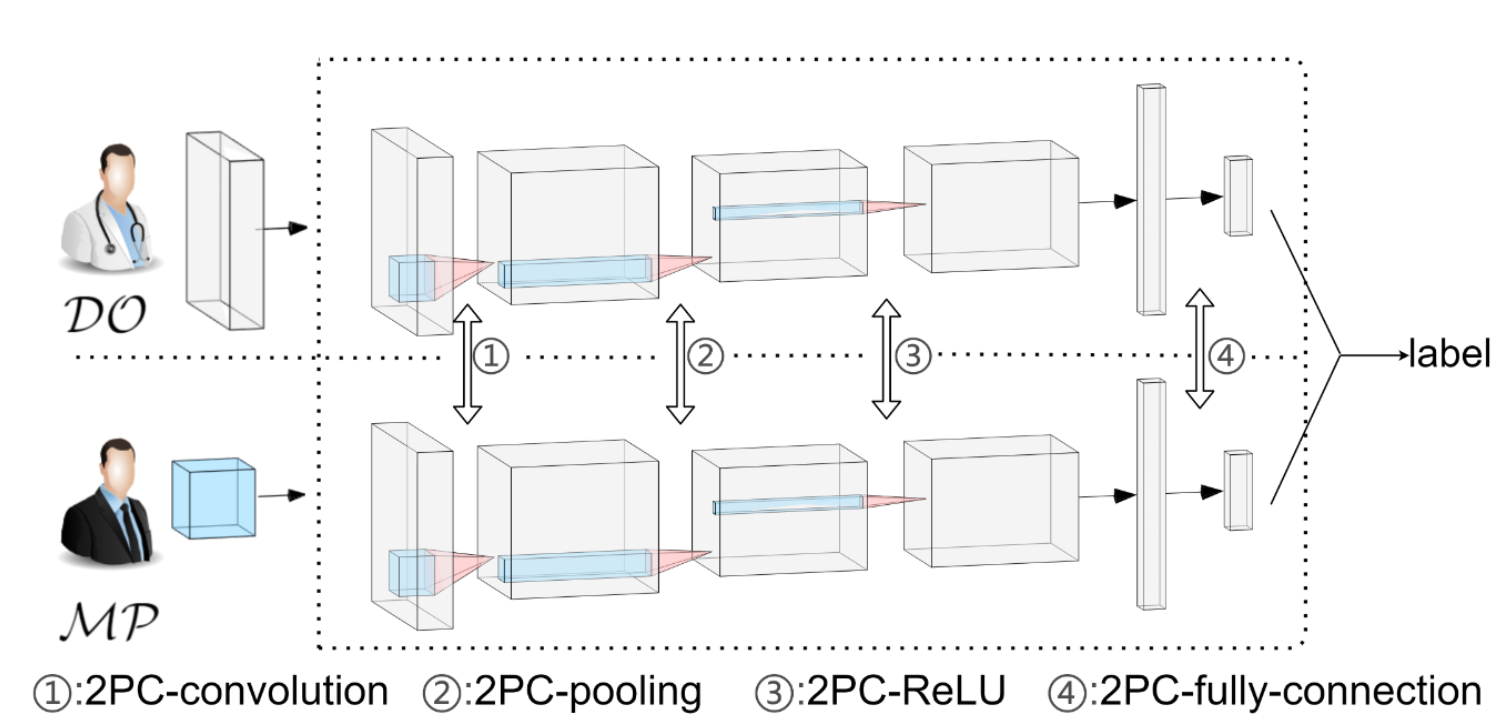
\includegraphics[width=8cm]{screenshot3.png}
        \caption{PrivNNP framework}
        \label{framework}
    \end{figure}
    As shown in Figure \ref{framework}, in our framework,
    the data owner ($\mathcal{DO}$) provides the input data
    and the model provider ($\mathcal{MP}$) provides the model parameters.
    $\mathcal{DO}$ and $\mathcal{MP}$ take the role of
    $\mathcal{P}_{0}$ and $\mathcal{P}_{1}$ to run 2PC protocols.
    After running the whole process of PrivNNP, they gather two shares of the prediction result and
    get the true value of the classification label.

\subsection{2PC neural network layers}
    Neural network has various architectures and
    most of these architectures are constructed of convolution layer,
    pooling layer, activation function layer, and other variant layers.
    We design the 2PC algorithms for these basic layers.



    \subsubsection{Convolution layer}


    When convolution is operated in practice,
    the input matrix $\mathbf{X}$ and weight tensor $\mathbf{W}$
    are rearranged into 2-dimension matrix $\mathbf{X}'$ and $\mathbf{W}'$.
    We denote this unrolling processing by
    $$(\mathbf{X}',\mathbf{W}')=\mathsf{Unroll} (\mathbf{X},W)$$
    Convolution can be converted into matrix multiplication and addition:
    $\mathbf{Y}=\mathbf{X}'\cdot \mathbf{W}'+\mathbf{B}'$, where $\mathbf{B}'$ is a matrix rearranged from the bias vector $\overrightarrow{\mathbf{b}}$ and
    $\mathbf{Y}$ is the output of convolution.
    Since the addition is easy to implement, we ignore the bias vector in this section by setting $\overrightarrow{\mathbf{b}}=\overrightarrow{0}$.
    So the convolution can be simplified to $\mathbf{Y}=\mathbf{X}'\cdot \mathbf{W}'$.
    % In order to elaborate better, we presents a mini-convolution to roughly show how this works.

    % When it comes to two-party secure computation,
    % $\mathcal{P}_{0}$ and $\mathcal{P}_{1}$ can locally
    % rearrange the shares of $\langle \mathbf{X}\rangle$ and $\langle \mathbf{W}\rangle$ to get
    % $(\langle \mathbf{X'}\rangle,\langle \mathbf{W'}\rangle)=\mathsf{Unroll}(\langle \mathbf{X}\rangle,\langle \mathbf{W}\rangle)$.
    Using $\mathtt{multiplication}$ protocol,
    two parties calculate $\langle \mathbf{Y}\rangle=\langle \mathbf{X'}\rangle\otimes \langle \mathbf{W'}\rangle$.
    This intuititive idea is not the best.
    \begin{figure}[htbp]
        \centering
        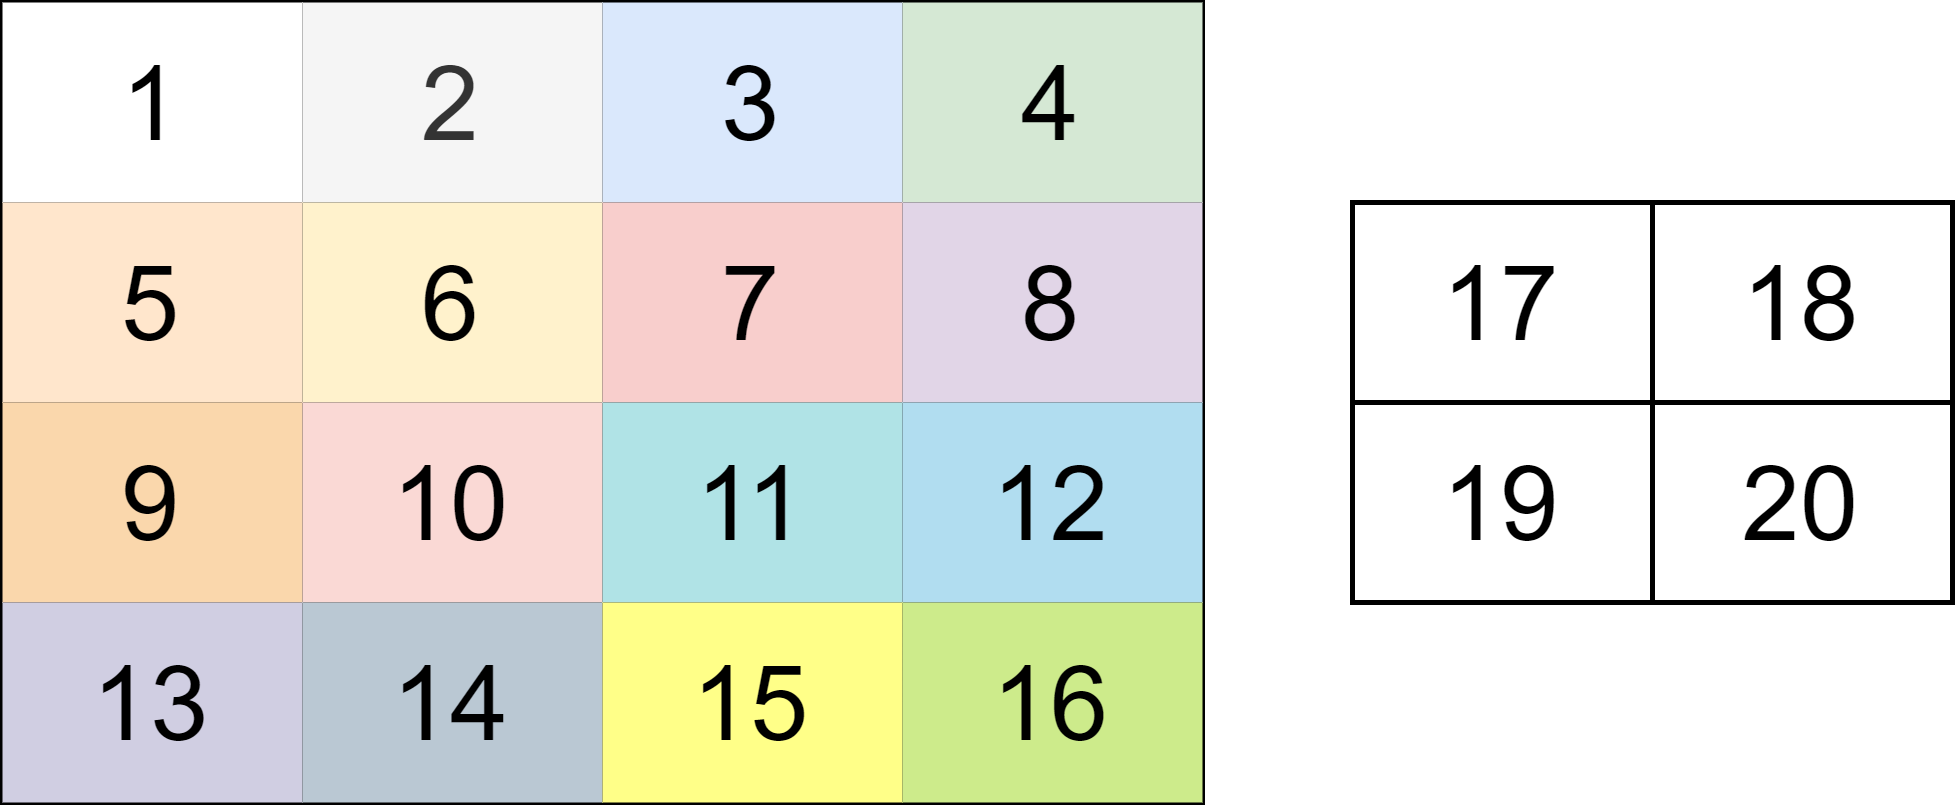
\includegraphics[width=4cm]{new_unrolling.png}
        \caption{Input matrix and weight}
        \label{input matrix and weight}
    \end{figure}

    Figure \ref{input matrix and weight} shows a mini-convolution,
    consisting of a $1\times 4\times 4$ input matrix $\mathbf{X}$  and a $1\times 2\times 2$ weight tensor $\mathbf{W}$.
    Each element of matrix is marked with different color and number.
    \begin{figure}[htbp]
        \centering
        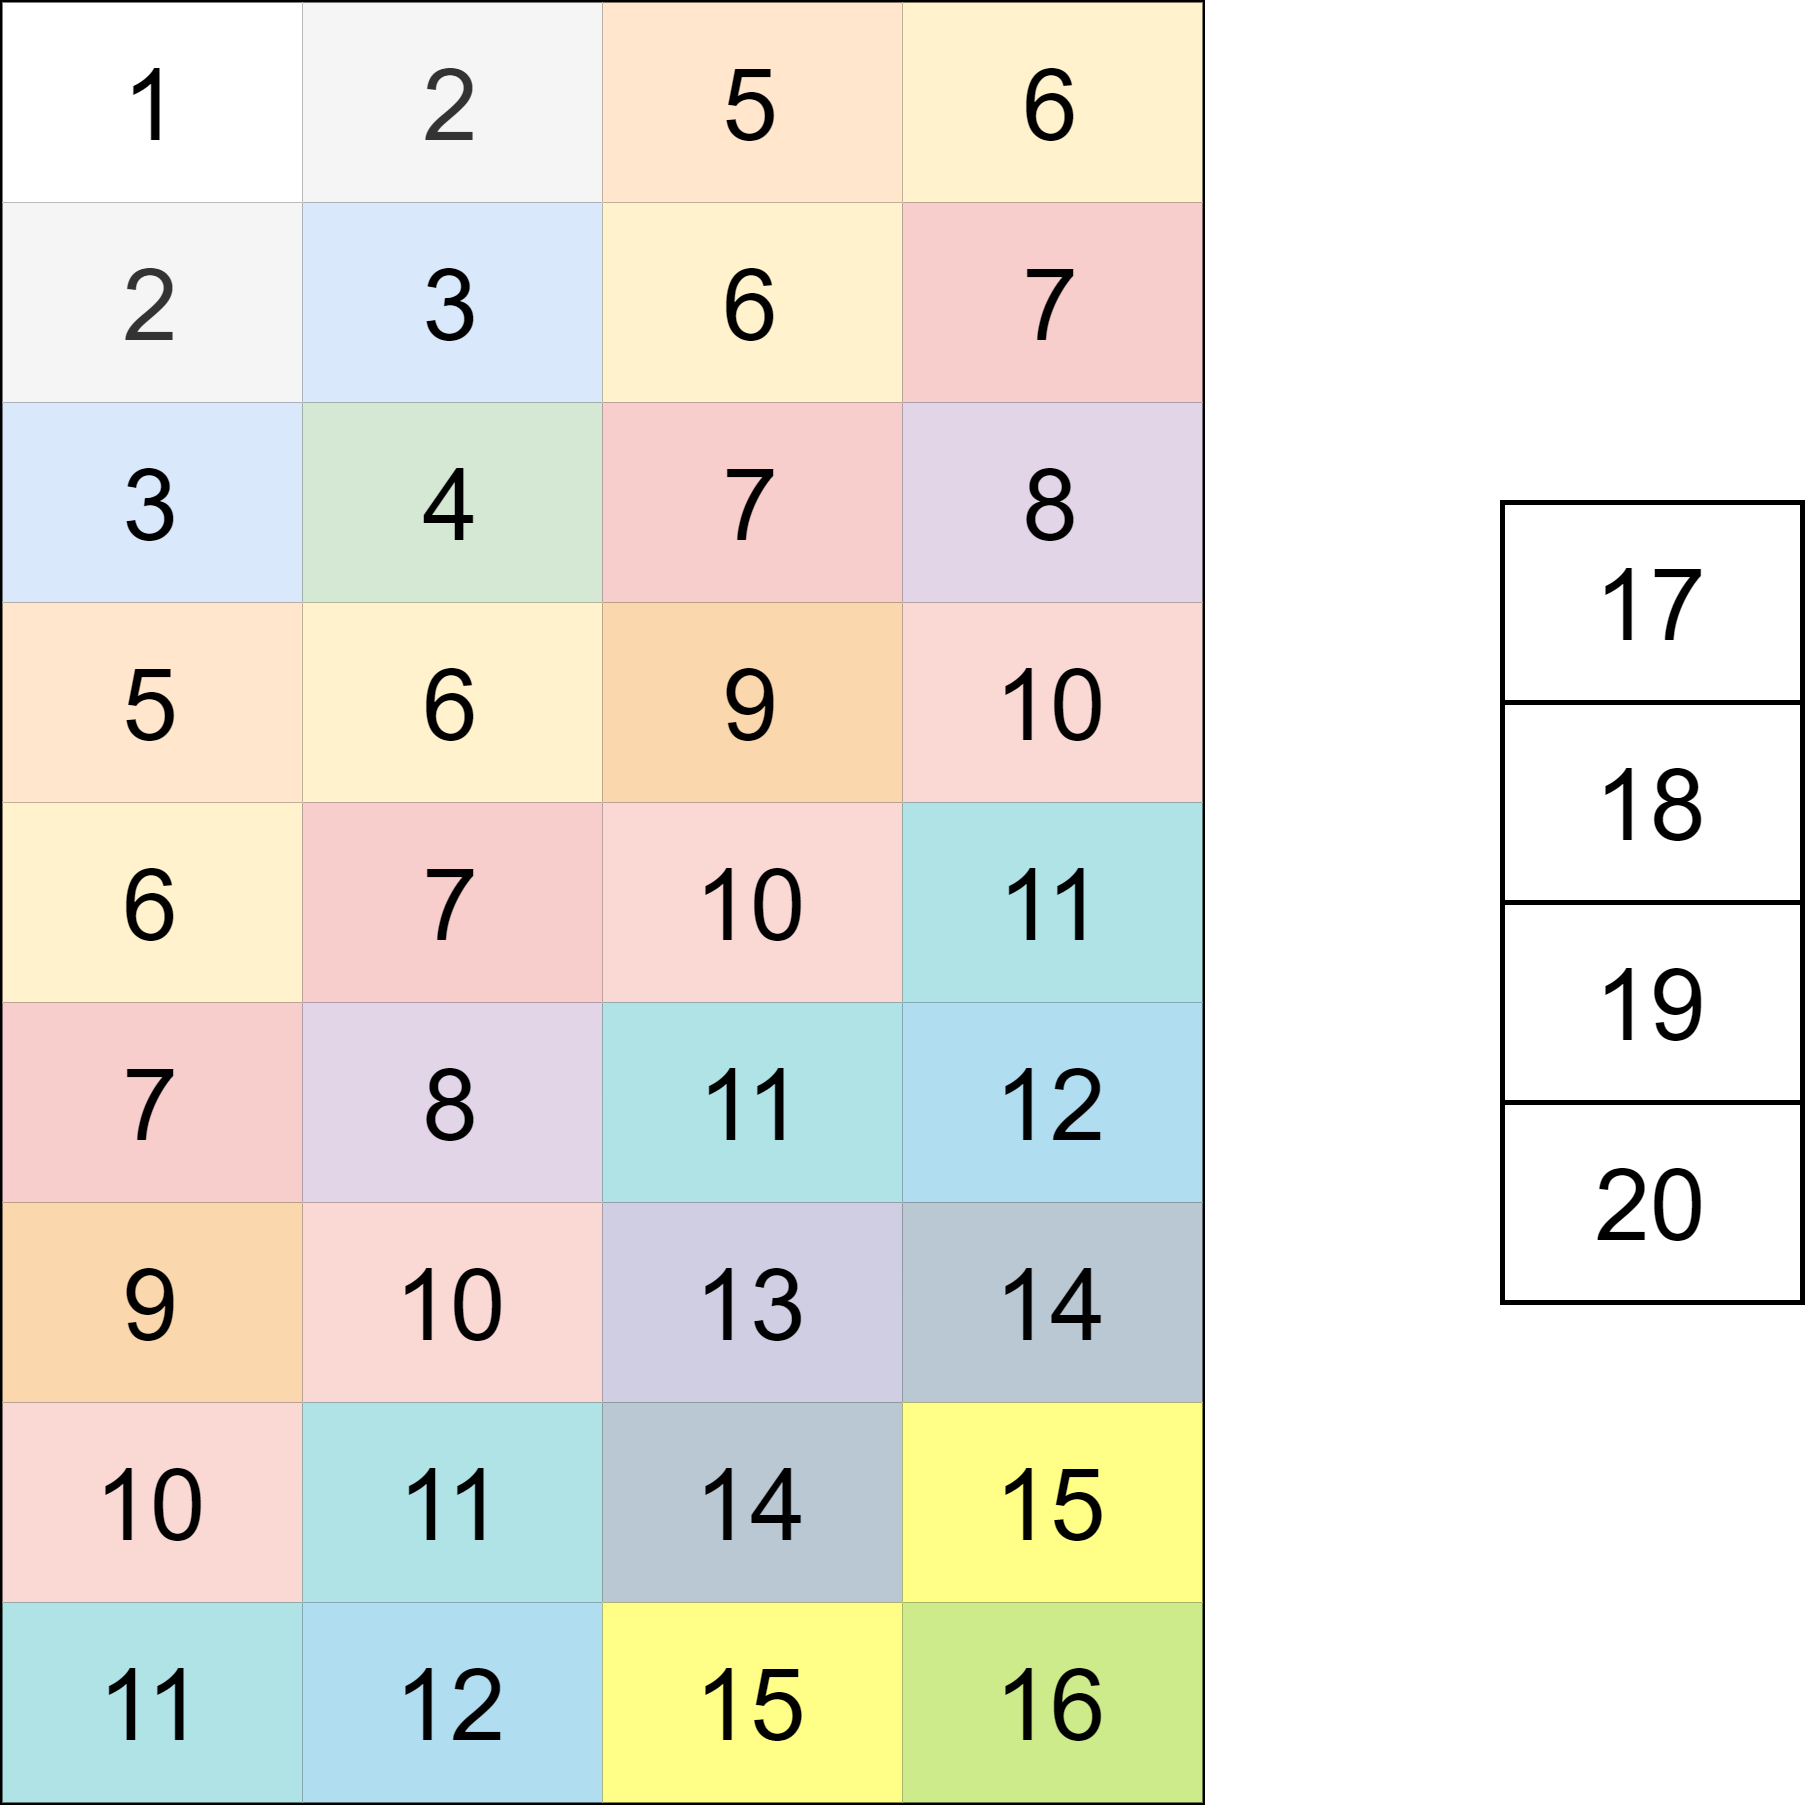
\includegraphics[width=4cm]{new_unrolling2.png}
        \caption{Rearranged matrix and weight}
        \label{rearrangement of matrix and weight}
    \end{figure}

    After rearrangement, matrix $(\mathbf{X}',\mathbf{W}')=\mathsf{Unroll}(\mathbf{X},\mathbf{W})$
    is shown in Figure \ref{rearrangement of matrix and weight}.
    Elements with blue font repeated four times
    and elements with red font were also duplicated two times.

    The duplicated element can be blinded by only one random number
    and two parties can  blind $(\mathbf{X},\mathbf{W})$ and
    construct the blinded $(\mathbf{X}',\mathbf{W}')$ locally instead of blinding $(\mathbf{X}',\mathbf{W}')$ directly.
    The optimization of 2PC-convolution is given below.


    % \begin{figure}
    %     \resizebox{0.48\textwidth}{!}{
    %     \begin{tabular}{lcl}
    %         \hline
    %         \multicolumn{3}{c}{\underline{$\mathtt{Matrix \enspace multiplication}$}:}\\
    %         \multicolumn{3}{l}{\textbf{Target}: compute $\langle \mathbf{Z}\rangle  = \langle \mathbf{X}\rangle  \otimes \langle \mathbf{Y}\rangle $}\\
    %         \textbf{Input}:\\
    %         % & \hfil\underline{$\mathtt{Multiplication}$}:\hfil\\
    %         $\mathcal{P}_{0}$ &  &  $\mathcal{P}_{1}$ \\
    %         $\{(\langle \mathbf{X}\rangle ^{0} , \langle \mathbf{Y}\rangle ^{0})\}$,
    %         &
    %         &
    %         $\{(\langle \mathbf{X}\rangle ^{1} , \langle \mathbf{Y}\rangle ^{1})\}$,
    %         \\
    %         % mul-triple:$
    %         % (\langle \mathbf{A}\rangle ^{0},\langle \mathbf{B}\rangle ^{0},\langle \mathbf{C}\rangle ^{0})\}$
    %         % &
    %         % &
    %         % mul-triple:$ (\langle \mathbf{A}\rangle ^{1},\langle \mathbf{B}\rangle ^{1},\langle \mathbf{C}\rangle ^{1})\}$
    %         \\
    %         \textbf{Procedure}:\\

    %         $\mathcal{P}_{0}$ &  &  $\mathcal{P}_{1}$ \\
    %         $\langle \mathbf{E}\rangle ^{0}\leftarrow\langle \mathbf{X}\rangle ^{0}-\langle \mathbf{A}\rangle ^{0}$
    %         &
    %         &
    %         $\langle \mathbf{E}\rangle ^{1}\leftarrow\langle \mathbf{X}\rangle ^{1}-\langle \mathbf{A}\rangle ^{1}$
    %         \\
    %         $\langle \mathbf{F}\rangle ^{0}\leftarrow\langle \mathbf{Y}\rangle ^{0}-\langle \mathbf{B}\rangle ^{0}$
    %         &
    %         &
    %         $\langle \mathbf{F}\rangle ^{1}\leftarrow\langle \mathbf{Y}\rangle ^{1}-\langle \mathbf{B}\rangle ^{1}$
    %         \\
    %         & $\underrightarrow{~~~~~~(\langle \mathbf{E}\rangle ^{0},\langle \mathbf{F}\rangle ^{0})~~~~~~}$ &\\
    %         & $\underleftarrow{~~~~~~(\langle \mathbf{E}\rangle ^{1},\langle \mathbf{F}\rangle ^{1})~~~~~~}$ &\\
    %         $e\leftarrow\langle \mathbf{E}\rangle ^{0}+\langle \mathbf{E}\rangle ^{1}$& &$\mathbf{E}\leftarrow\langle \mathbf{E}\rangle ^{0}+\langle \mathbf{E}\rangle ^{1}$\\
    %         $f\leftarrow\langle \mathbf{F}\rangle ^{0}+\langle \mathbf{F}\rangle ^{1}$& &$\mathbf{F}\leftarrow\langle \mathbf{F}\rangle ^{0}+\langle \mathbf{F}\rangle ^{1}$\\
    %         $\langle \mathbf{Z}\rangle^{0}\leftarrow \mathbf{F}\cdot \langle \mathbf{A}\rangle^{0}$
    %         & &
    %         $\langle \mathbf{Z}\rangle^{1}\leftarrow \mathbf{E} \cdot \mathbf{F} + \mathbf{F}\cdot \langle \mathbf{A}\rangle^{1}$\\
    %         $+\mathbf{E} \cdot \langle \mathbf{B}\rangle^{0} + \langle \mathbf{C}\rangle^{0}$& &$+\mathbf{E} \cdot \langle \mathbf{B}\rangle^{1} + \langle \mathbf{C}\rangle^{1}$\\
    %         \hline

    %     \end{tabular}}
    %     \caption{2PC-convolution}
    %     \label{2PC-convolution}


    % \end{figure}

    \textbf{Protocol procedure}:
    \begin{itemize}
        \item \textbf{1.} $TTP$ randomly chooses the matrix $(\mathbf{A},\mathbf{B})$ of the same size
        as the original feature $\mathbf{X}$ and the filter weight $\mathbf{W}$.
        \item \textbf{2.} $TTP$ evaluates $( \mathbf{A}',\mathbf{B}')=\mathsf{Unroll}(\mathbf{A},\mathbf{B})$
        and $\mathbf{C}' =\mathbf{A}'\cdot \mathbf{B}' $.
        Then, $TTP$ sends $(\langle \mathbf{A}\rangle ^{i},\langle \mathbf{B}\rangle ^{i},\langle \mathbf{C}'\rangle ^{i})$
        to $\mathcal{P}_{i}$.
        \item \textbf{3.} $\mathcal{P}_{i}$ sets $\langle \mathbf{E}\rangle ^{i}=\langle \mathbf{X}\rangle ^{i}-
        \langle \mathbf{A}\rangle ^{i}$
        and $\langle \mathbf{F}\rangle ^{i}=\langle \mathbf{W}\rangle ^{i}-\langle \mathbf{B}\rangle ^{i}$
        and transmits $(\langle \mathbf{E}\rangle ^{i},\langle \mathbf{F}\rangle ^{i})$ to $\mathcal{P}_{1-i}$.
        \item \textbf{4.} $\mathcal{P}_{i}$ reconstructs $\mathbf{E} = \langle \mathbf{E}\rangle ^{0}+\langle \mathbf{E}\rangle ^{1}$,
        $\mathbf{F} = \langle \mathbf{F}\rangle ^{0}+\langle \mathbf{F}\rangle ^{1}$
        and rearranges $(\mathbf{E}',\mathbf{F}')=\mathsf{Unroll}(\mathbf{E},\mathbf{F})$ and $(\mathbf{A}',\mathbf{B}')=\mathsf{Unroll}(\mathbf{A},\mathbf{B})$.
        \item \textbf{5.} $\mathcal{P}_{i}$ sets
        $\langle \mathbf{Z}\rangle^{i}=i\cdot \mathbf{E}' \cdot \mathbf{F}' +
        \langle \mathbf{A}'\rangle^{i} \cdot \mathbf{F}' + \mathbf{E}' \cdot \langle \mathbf{B}'\rangle^{i} + \langle \mathbf{C}'\rangle^{i}$.

    \end{itemize}
    By this way, communication overhead can be reduced to almost $ \frac{1}{width^{2}} $ of the original,
    where $width$ is the width of the filter.


    \subsubsection{Pooling layer}


    There are two types of pooling layer: average pooling and maximum pooling,
    which output the average or the maximum of $n\times n$ size submatrices respectively
    to construct the input matrix of next layer.
    We take $2\times 2$ window as an example to show how $\mathcal{P}_{0}$ and $\mathcal{P}_{1}$ compute the output of a submatrix.
    For each $2\times 2$ submatrix $\mathbf{X}$, average pooling outputs $y_{avg}=\frac{X_{00}+ X_{01}+ X_{10}+  X_{11}}{4}$
    and maximum pooling outputs $y_{max}=\mathsf{max}(X_{00}, X_{01}, X_{10},  X_{11})$
    $$  \langle \mathbf{X}\rangle ^{0}= \begin{bmatrix}
        \langle X_{00}\rangle ^{0}& \langle X_{01}\rangle ^{0} \\
        \langle X_{10}\rangle ^{0}& \langle X_{11}\rangle ^{0}
       \end{bmatrix}\langle \mathbf{X}\rangle ^{1}=\begin{bmatrix}
        \langle X_{00}\rangle ^{1}& \langle X_{01}\rangle ^{1} \\
        \langle X_{10}\rangle ^{1}& \langle X_{11}\rangle ^{1}
       \end{bmatrix}$$

    2PC-average pooling is easy to implement by local division.
    To get the average of elements in submatrix $\mathbf{X}$,
    $\mathcal{P}_{0}$ sets $\langle y_{avg}\rangle^{0} = \frac{\langle X_{00}\rangle ^{0}+ \langle X_{01}\rangle ^{0}+
    \langle X_{10}\rangle ^{0}+ \langle X_{11}\rangle ^{0}}{4}$ and
    $\mathcal{P}_{1}$ sets $\langle y_{avg}\rangle^{1} = \frac{\langle X_{00}\rangle ^{1}+ \langle X_{01}\rangle ^{1}+
    \langle X_{10}\rangle ^{1}+ \langle X_{11}\rangle ^{1}}{4}$. This process can be done without interaction.

    2PC-maximum pooling layer can be computed by recursively running $\mathtt{comparison}$ protocol.
    % The approach has been briefly discussed before and now we give it in detail.
    Consider that
    \begin{align*}
        y_{max} &= \mathsf{max}(X_{00}, X_{01}, X_{10}, X_{11}) \\
        &= \mathsf{max}(\mathsf{max}(X_{00},X_{01}),\mathsf{max}( X_{10}, X_{11}))
    %     &= \mathsf{max}(X_{00},\mathsf{max}(X_{01}, X_{10}, X_{11})) \\
    %   &= \mathsf{max}(X_{00},\mathsf{max}(X_{01},\mathsf{max}(X_{10}, X_{11})))
    \end{align*}
    So the maximum of each submatrix can be obtained by running
    maximum protocol for three times.
    After repeating this process to each submatrix, parties can get the output matrix of the pooling layer.


    \subsubsection{Activation function layer}
    Here we explore one  activation function: $\mathsf{ReLU}()$, a typical continuous piecewise function.
    % which can be calculated referring to piecewise function protocol in 3.4.
    $$\mathsf{ReLU}(x)=\begin{cases}
        0 & \text{ if } x \leqslant 0  \\
        x & \text{ if } x > 0
        \end{cases}$$
    $\mathsf{ReLU}$ function has three dividing points: $d_{0}= -\infty ,d_{1}= 0, d_{n}=+\infty$ and two sub-functions:
    $\mathsf{f}_{1}(x)= 0 ,\mathsf{f}_{2}(x)= x$.
    With $v_{j} = (1-\mathsf{sign}(d_{j-1}-x)\cdot \mathsf{sign}(d_{j}-x))/2$, this function can be represented as
    % $$\mathsf{ReLU}(x)=\sum_{j=1}^{2}v_{j}\cdot \mathsf{f}_{j}(x)=v_{1}\cdot \mathsf{f}_{1}(x)+v_{2}\cdot \mathsf{f}_{2}(x)=v_{1}\cdot 0 +v_{2}\cdot x=v_{2}\cdot x$$
    \begin{align*}
        \mathsf{ReLU}(x)&=\sum_{j=1}^{2}v_{j}\cdot \mathsf{f}_{j}(x)=v_{1}\cdot \mathsf{f}_{1}(x)+v_{2}\cdot \mathsf{f}_{2}(x)\\
        &=v_{1}\cdot 0 +v_{2}\cdot x\\
        &=\frac{(1-\mathsf{sign}(d_{1}-x)\cdot \mathsf{sign}(d_{2}-x))\cdot x}{2} \\
        &=\frac{(1-\mathsf{sign}(0-x)\cdot \mathsf{sign}(+\infty -x))\cdot x}{2} \\
        &=\frac{(1+\mathsf{sign}(x))\cdot x}{2}
    \end{align*}

    Parties can follow $\mathtt{multiplication}$ protocol and $\mathtt{comparison}$ protocol to compute
    $\langle y\rangle=\langle \mathsf{ReLU}(\langle x\rangle)\rangle=\frac{(1+\langle \mathsf{sign}(\langle x\rangle)\rangle)\otimes \langle x\rangle}{2}$.
    Other activation functions like $\mathsf{Sigmoid}$ can be evaluated by
    approximate piecewise functions.


    \section{Theoretical Analysis}
    \begin{table}[!ht]

        % \center
        \resizebox{0.45\textwidth}{!}{
        \begin{tabular}{|c|c|c|c|c|}\hline

        \multirow{2}{*}{2PC task}& \multirow{2}{*}{schemes} &asymmetric & communication & \multirow{2}{*}{rounds}     \\
        &   &    computation       &     (floating-points)      &            \\ \hline
        \multirow{3}{*}{comparison}&ABY&                   18$l$& $7l\cdot \kappa+(l^{2}+l)/2$ &6\\\cline{2-5}
        &Sharemind&               0&     6$l$               &$l$\\\cline{2-5}
        &PrivNNP&                   0&   5                  &3 \\\hline

        &ABY&                   54$l$& $21l\cdot \kappa+(l^{2}+l)3/2+12$ &16\\\cline{2-5}
        pooling&Sharemind&               0&     18$l$ +12              &$2l+4$\\\cline{2-5}
        &PrivNNP&                   0&   27                  &10 \\\hline

        \multirow{3}{*}{ReLU}&ABY&                   18$l$& $7l\cdot \kappa+(l^{2}+l)/2+2$ &7\\\cline{2-5}
        &Sharemind&               0&     $6l+2$             &$l+1$\\\cline{2-5}
        &PrivNNP&                   0&   7                  &4 \\\hline


        \end{tabular}}
        \caption{Overhead of different 2PC schemes with $l$-bits value inputs }
        \label{Overhead of methods}
    \end{table}
    Overhead of 2PC algorithms including
    ABY, Sharemind and PrivNNP
    for comparison, maximum pooling
    and ReLU function is shown in Table \ref{Overhead of methods}.
    PrivNNP performs best in all respects.


    % The biggest advantage of PrivNNP is that we design a novel $\mathtt{comparison}$ protocol which has
    % a huge improvement over the previous work.
    % We list the state-of-art 2PC-$\mathtt{comparison}$ protocol:
    % ABY and Sharemind, and compare them to our work.
    % As shown in Table \ref{Overhead of methods}, asymmetric cryptographic computation, communication bits and
    % interaction rounds are listed.
    % Obliviously, our scheme shows the best performance.


    \section{Experimental result}
    To evaluate the performance of our work, we conduct simulation experiments on a desktop (CPU: AMD Ryzen 7 5800H with 3.20GHz).
    We use two independent folders placed on different physical hard drives to simulate two servers belonging to the
    data owner and the model provider for measuring the time cost of computation.
    % and we calculate the communication consumption by counting all of floating-point numbers needed to be passed.
    We use Python 3.9.7 to implement our system and use functions in the SPDZ library \cite{SPDZ}.
    All operations involved in the experiments are floating-point operations.
    Files are written in form of npy format supported by Python, where a floating-point number occupies about 0.0078Kb.
    For accurate and stable measurement, file transfer rate between servers is fixed at 10M/s.
    Each experiment was repeated 10 times.

    The experiments are divided into three parts basic operations neural network layers and neural network implementation.
    \subsection{Operations}
    \begin{figure}[htbp]
        \subfigure[multiplication] %第一张子图
        {
            \begin{minipage}{0.45\linewidth}
                \centering
                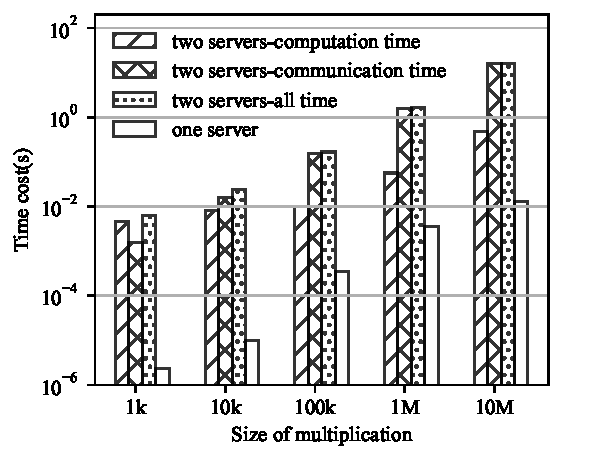
\includegraphics[width=4cm]{operation_mul.pdf}
                % \caption{operation mul}
                \label{operation_mul}
            \end{minipage}
        }
        \subfigure[matrix multiplication] %第二张子图
        {
            \begin{minipage}{0.45\linewidth}
                \centering
                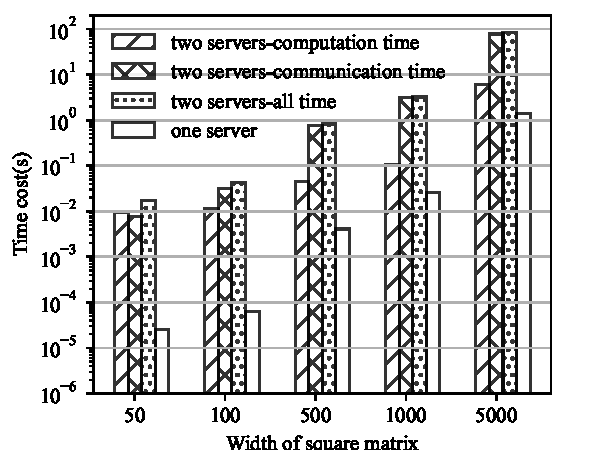
\includegraphics[width=4cm]{operation_matrix_mul.pdf}
                % \caption{operation matrix mul}
                \label{operation_matrix_mul}
            \end{minipage}
        }
        \caption{Experiment I-Overhead of 2PC-multiplication and matrix multiplication}
        \label{multiplication and matrix multiplication}

    \end{figure}

    \begin{figure}[htbp]

        \centering
        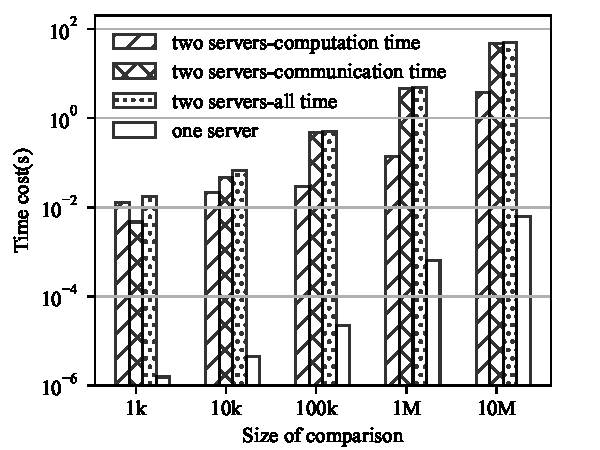
\includegraphics[width=5cm]{operation_compare.pdf}
        \caption{Experiment I-Overhead of 2PC-comparison}
        \label{operation_compare}
    \end{figure}
    In Experiment I, time consumption of basic operations including multiplication, comparison and matrix multiplication are measured.
    % Experiment results of multiplication and matrix multiplication are shown in \ref{operation_mul}
    For benchmark test, we give the time consumption of one server operating directly as a reference.
    The data obtained is shown in Figure \ref{multiplication and matrix multiplication} and Figure \ref{operation_compare}.

    The time cost of secure two-party calculation is divided into two parts:
    local calculation and online communication.
    the time consumption of online communication increases linearly with the increase of the number of elements,
    while local computation time is more complicated.
    There will be a lot of fixed time consumption of calling system file functions
    for file writing and reading operations.

    The three operations show the same trend that
    when the number of elements achieves 10k and more,
    the communication time becomes longer than the calculation time.
    Take matrix multiplication as an example,
    when the width is $1000$, the communication costs $3.12$s, accounting for $96\%$ of total time.

    \subsection{Neural network layers}
    In Experiment II, overhead of neural network layers including
    convolution layer, pooling layer and $\mathsf{ReLU}$ function are measured.

    \begin{table}[!ht]

        \center
        \resizebox{0.45\textwidth}{!}{
        \begin{tabular}{|c|c|c|c|c|c|}\hline

        \multicolumn{6}{|c|}{Convolution Layer}\\ \hline
        \multirow{2}{*}{feature size}&\multirow{2}{*}{size of filter}& \multicolumn{3}{c|}{cost time(s)}&communication \\

        \cline{3-5}
        \multirow{2}{*}{ }&\multirow{2}{*}{ }&computation&communication&all&size(Mb)  \\ \hline
        (64,56,56)& (64,64,3,3) & 0.64  & 0.18 & 0.82 &0.28\\ \hline
        (256,28,28)& (512,256,1,1) & 0.48 & 0.26 & 0.74 & 0.16 \\ \hline
        (256,14,14)& (256,256,3,3) & 0.20 & 0.50 & 0.70 & 0.096\\ \hline
        (1024,7,7)& (2048,1024,1,1) & 0.21 & 1.68 & 1.89 & 0.086 \\ \hline \hline

        \multicolumn{6}{|c|}{Pooling Layer}\\ \hline
        \multicolumn{2}{|c|}{\multirow{2}{*}{feature size}}& \multicolumn{3}{c|}{cost time(s)}&communication   \\

        \cline{3-5}
        \multicolumn{2}{|c|}{}&computation&communication&all&size(Mb)\\ \hline
        \multicolumn{2}{|c|}{(256,14,14)} & 0.088  & 0.26 & 0.35 &2.6	\\ \hline
        \multicolumn{2}{|c|}{(256,28,28)} & 0.107 & 1.05 & 1.16 & 10.5 \\ \hline
        \multicolumn{2}{|c|}{(256,56,56)} & 0.240  & 4.23 & 4.47 &42.3	\\ \hline
        \multicolumn{2}{|c|}{(256,112,112)} & 0.746 & 16.93 & 17.68 & 169.3 \\ \hline          \hline

        \multicolumn{6}{|c|}{ReLU}\\ \hline
        \multicolumn{2}{|c|}{\multirow{2}{*}{feature size}}& \multicolumn{3}{c|}{cost time(s)}&communication   \\

        \cline{3-5}
        \multicolumn{2}{|c|}{} &computation&communication&all&size(Mb)\\ \hline
        \multicolumn{2}{|c|}{(256,14,14)} & 0.025  & 0.27 & 0.29 &2.7	\\ \hline
        \multicolumn{2}{|c|}{(256,28,28)} & 0.054 & 1.09 & 1.15 & 10.9 \\ \hline
        \multicolumn{2}{|c|}{(256,56,56)} & 0.160  & 4.39 & 4.55 &43.9	\\ \hline
        \multicolumn{2}{|c|}{(256,112,112)} & 0.631 & 17.56 & 18.19 & 175.6 \\ \hline

        \end{tabular}}

        \caption{Experiment II-Layers consumption}
        \label{Layers_consumption}
    \end{table}


    For different neural network layers,
    % we select several representative shapes of features and filters
    % to test the time cost.
    the result is shown in Table \ref{Layers_consumption}.
    In general, the computational overhead of neural network layers has been reduced to an acceptable range
    and the communication cost still account for the vast majority.




    \subsection{Neural networks}
    In Experiment III, we conduct
    time-consuming tests on a small network Lenet-5 \cite{Lenet5} and a large network Resnet50\cite{DeepResidualLearning}.
    The MNIST dataset is used for training neural network models, which consists of about 70000 images of size $1\times 28 \times 28$ with $10$ classes
    for handwriting recognition.
    Since the size of input image of Resnet50 is $3\times 224 \times 224$,
    we resize each image of MNIST dataset to $3\times 224 \times 224$ for training the Resnet50 model.
    Notably, we remove the batch normalization layers of Resnet50 because PrivNNP
    cannot implement the division of which the dividsor is a secret variable.


    \begin{table}[!ht]
        \center
        \resizebox{0.45\textwidth}{!}{
        \begin{tabular}{|c|c|c|c|c|}\hline
        \multirow{2}{*}{model}& \multicolumn{3}{c|}{time(s)}&communication  \\
        \cline{2-4}
        \multirow{2}{*}{ }&computation&communication&all&size(Mb) \\ \hline
        Lenet-5 & 0.375  & 0.32 & 0.69 &3.2	\\ \hline
        Resnet50 & 23.85 & 100.13 & 123.98 & 1001.3 \\ \hline
        \end{tabular}}
        \caption{Experiment III-Neural networks consumption}
        \label{neural networks consumption}
    \end{table}

    As shown in Table \ref{neural networks consumption}, PrivNNP shows an excellent performance
    both in medium and large neural networks.
    A prediction of Resnet50 costs 23.85s for computation and 100.13s for communication.

    \section{Conclusion and Future Work}
    In this work, we presented PrivNNP, a two-party computation framework for neural network predictions.
    This framework is based on a novel 2PC-$\mathtt{comparison}$ protocol which does not involve asymmetric cryptographic operations
    and we design methods to evaluate each layer in neural network and implement an experiment on Resnet50.
    This framework has great potential
    since we only consider the WAN setting where the communication speed is limited.
    Future work can utilize the LAN to reduce the communication time cost.
\bibliography{aaai23}


% \bibentry{ABY3}
% \bibentry{ABY}
% \bibentry{EfficientMultipartyProtocols}
% \bibentry{ChironCloud}
% \bibentry{HighPerformanceConvolutional}
% \bibentry{ObliviousNeuralNetwork}
% \bibentry{DeepResidualLearning}
% \bibentry{MaliciouslySecureMatrixMultiplication}
% \bibentry{CryptoNets}
% \bibentry{Sharemind}
% \bibentry{Homomorphic1}
% \bibentry{Homomorphic2}
% \bibentry{Lenet5}
% \bibentry{}
% \bibentry{}
% \bibentry{}
% \bibentry{}
% \bibentry{}
% \bibentry{}


\end{document}

